\begin{frame}{\alert{Tâche} : synthèse}
\begin{center}

\includegraphics[width=.3\columnwidth]{figures/play}
\end{center}
\end{frame}

tache synthèse

attrait personnel
challenge
en prise avec les problématiques actuelles en apprentissage

problème de formalisation

requis qualitatif

prototype fonctionnel

apprentissage non supervisé


\begin{frame}{Court terme}
\begin{description}
\item[Félix Gontier]: inversion de features pour la synthèse de scènes sonores respectueuses de la vie privée (ANR Cense)
\item[Tom Souaille]: conception interactive en design sonore (Ouest Industrie Créatives)
\end{description}
\end{frame}

\begin{frame}{Moyen terme}
\begin{itemize}
\item inversion de l'opérateur de diffusion d'ondelettes
\item synthèse audio neuronale
\item en particulier les approches basées échantillons
\end{itemize}
\end{frame}

\begin{frame}{Déplacements US}
\begin{block}{Côte ouest}
\begin{itemize}
\item Jesse Engels, magenta, Google brain (SFB)
\item Justin Salamon, audio research group, Adobe research (SFB)
\end{itemize}
\end{block}
\begin{block}{Côte est}
\begin{itemize}
\item Juan Pablo Bello, music and audio research group, NYU (NY) 
\item Mounya Elhilali, Laboratory for Computational Audio Perception, Johns Hopkins University (Baltimore)
\item Joakim Andèn, Flatiron Institute (NY)
\end{itemize}
\end{block}
\end{frame}

\begin{frame}{Long terme}
\begin{center}
 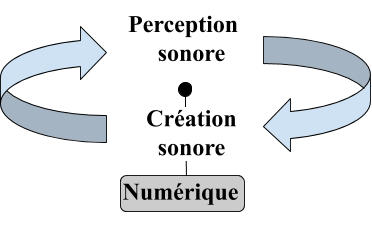
\includegraphics[width=.6\columnwidth]{longTerme}
\end{center}
\begin{description}
\item[comprendre] : mesure et qualification de l'environnement sonore et de sa perception
\item[innover] : 
\begin{itemize}
\item Andy Hildebrand (Autotune)
\item Xavier Serra (Vocaloïd)
\end{itemize}
\end{description}
\end{frame}

\begin{frame}{Contributions}
\small
Publications
\begin{itemize}
\item \fullcite{lagrangeTaslp06}
\item \fullcite{lagrangeTaslp08}
\item \fullcite{lafayhal-01111381}
\end{itemize}
Logiciels
\begin{itemize}
\item \fullcite{explanes}
\item \fullcite{simscene}
\end{itemize}
\end{frame}


\begin{frame}{Figure}
\begin{center}

\includegraphics[width=.6\columnwidth]{figures/play} \\
\end{center}
\end{frame}

\begin{frame}{Block}
\begin{block}{title}
\begin{itemize}
\item
\item
\item
\end{itemize}
\end{block}
\end{frame}


\begin{frame}{Itemize}
\begin{itemize}
\item
\item
\item
\end{itemize}
\end{frame}